\chapter{Introduction}\label{ch1}


%%%% Currently

% Rewrote introduction based on talk with steven
%%% Neeed to
% Rewrite hypothesis
% Edit and reform paragraphs of introductory text so that the story is clear, makes sense and has references



%Introduction+conclusion are shorter chapters

%Introduction
%Hypothesis
%research questions
%context
%Summary of the contributions
%Good to introduce gently but research questions can be fine
%Doesn't have to be accessible to the man on the street, need computer science background, vector spaces are included in that, so are decision trees and neural networks, if it's borderline reference background

%%Conclusion revisits research questions, provides the answer not just a summary

%%%%% INTRODUCTION

% There is a lot of data, and a lot of good applications of machine-learning using that data




%!!!!!!!!!!!!!!! NEW INTRO


%  There is a lot of data available, and even more becoming so, so machine-learning that  leverages this data are getting top performance on a lot of tasks.
% Neural networks are not interpretable, Interpretable classifiers are useful because they can drive engagement, increase stakeholder buy in, inform model creators of errors or ways to improve the model, provide insight
% A successful interpretable classifier 1. Uses features that correspond to key domain concepts, and 2. Explains what these concepts represent, as well as the decision made with these concepts 
% we aim to satisfy the first objective, but are not interested in obtaining labels or explanations based on these labels. So, we obtain features that correspond to meaningful and specific concepts that are relevant to classifying key domain tasks For example, when classifying "horror" a good feature would be how "bloody" the movie is., 
% In particular, this work investigates interpretable classifiers for document classification. For example, genres in a domain of movie reviews.
%% Machine learning uses spatial representations of meaning, and neural networks can be seen as constructing such a spatial representation of meaning. 
%This thesis focuses on transforming vector space representations into semantic features in an unsupervised way.    These are obtained from stevens and derrac's method, and are used as directions,  they have previously been found to be   suitable for different applications, like a recommendation system where you can choose something that's "more bloody"



% Move disentanglement to background?, defining disentanglement paper

%\hmark{Typically, to obtain a representation that represents meaningful aspects of the domain, a low-dimensional vector space representation is induced. However, in these representations the features do not correspond to meaningful aspects, but rather this meaning is represented spatially.}   %The problem with these vector spaces is that despite the fact that these representations clearly capture meaning in a non-trivial way,  their features do not typically have any particular meaning. %Ideally, a representation  of documents   is flexible in the information it can represent, and is learned from a large amount of data. To do this, typically Low-dimensional vector space embeddings of documents represent semantic meaning spatially.

% Machine-learning methods can achieve strong results, but are not interpretable.


%  There is a lot of data available, and even more becoming so, so machine-learning that  leverages this data are getting top performance on a lot of tasks.
%  This is in-part thanks to the availability of  text data on the internet, as  social media sites  like Facebook and  Twitter, \hmark{p}roduct and movie review sites like IMDB and Amazon and content-aggregation sites like Reddit have become immensely popular. % , or text classification tasks . \hmark{Some examples of these text classification tasks are} and text classification tasks \cite{Burel2018, Aldarwish2017, Burel2018}. e.g.\  identifying if social media posts or product reviews have a positive or negative sentiment,  identifying social media posts  that are useful to crisis responders during crises, or  predicting depression in social media users. 

% Neural networks are not interpretable, Interpretable classifiers are useful because they can drive engagement, increase stakeholder buy in, inform model creators of errors or ways to improve the model, provide insight
\hmark{In recent years, machine learning models  have  achieved state-of-the-art results on most natural language processing tasks\footnote{https://github.com/sebastianruder/NLP-progress} such as machine translation, \cite{Wu} question answering  \cite{Fisch2016}, and document classification \cite{Yang2019}. % in part thanks to the ability of these models to process  large amounts of unstructured text data made widely available by the internet.
Although these methods perform well, they are typically not interpretable. As machine learning has extended into  real-world domains like medicine and policing, concerns of safety \cite{Amodei2016} and fairness \cite{Mehrabi2019} have brought  the  legality and risk of implementing systems that are not interpretable   to the attention of lawmakers. The European Union introduced  a legal "Right to explanation" in 2018   \cite{Goodman2016}, requiring that machine learning models must be able to explain why they have made a decision about a person. }
%A variety of solutions have Solutions such as explaining machine-learning models after they have been learned have been suggested, as well as making transparent machine-learning models that can be understood by inspection \cite{Gilpina}. 

% A successful interpretable classifier 1. Uses features that correspond to key domain concepts, and 2. Explains what these concepts represent, as well as the decision made with these concepts  we aim to satisfy the first objective, but are not interested in obtaining labels or explanations based on these labels. So, we obtain features that correspond to meaningful and specific concepts that are relevant to classifying key domain tasks For example, when classifying "horror" a good feature would be how "bloody" the movie is., 

\hmark{Simple interpretable models are one solution to this problem. A prototypical example of a simple interpretable model is a low-depth decision tree. This low-depth decision tree can be used as a classifier model, in the  NLP task of document classification, the task of assigning  text documents to distinct classes. In order to use text documents as  input to a low-depth decision tree, they must be first processed into a mathematical representation. One standard way to obtain a representation of  a collection of text documents is using the  bag-of-words model. The bag-of-words model takes the form of a matrix where each row corresponds to a text document and each column corresponds to a word in the corpus. The value  of a word for a document would be the frequency of the word in that document, as a standard example.} %This representation is necessarily sparse, and each feature (i.e.\ word) that is used to represent a document can be inspected and understood.


% There are two goals, semantic features and interpretable labels
% Bag-of-words have interpretable labels but not semantic features
% Ideally semantic features will correspond to concepts that can be used to classify the class
% Semantic representations encode these concepts spatially, but do not represent them as features

\hmark{One domain investigated in this thesis is the 20 newsgroups domain, where forum topics are text documents. These forum topics are composed of user text posts, and  each topic is submitted to separate categories. In this domain, a document classification task is to assign documents (forum topics) to the categories they originated from (e.g.\ automobiles, computer-science). In-order for a low-depth decision tree to perform well on this task, the features must capture properties in the domain related to these categories.  As an extreme example, in  a decision tree limited to a depth of one,  a single feature is used. For this decision to perform well, e.g.\ by classify if a topic is from the "automobile" category,  the feature used must  capture a property that is highly related to "automobiles". This feature would have a high value if the text document (i.e.\ topic) is highly related to automobiles, and a low value on the feature if  the document is not related to automobiles.} %This would allow the decision tree to find a boundary that separates  text documents that are related to automobiles from those that aren't.

\hmark{In this task, the bag-of-words representation can represent a variety of words that are relevant only to automobiles, e.g.\ "car", "diesel", "volkswagen", or even "automobile". However, the bag-of-words is necessarily sparse, and requires a deep tree that can include many relevant features for good classification performance. As an example, in a one-depth decision tree, making a classification decision based on the frequency of the word "automobile" will likely identify posts that are related to automobiles, but will also miss many posts that are related but do not contain this word.}  

\hmark{A bag-of-words can be used as input to a dimensionality reduction method to be obtain a vector space. After this process, each document is represented as a vector, where the number of dimensions is far lower than the number of features in the bag-of-words representation. As an example, in the domain of newsgroup postings, topics that are similar, for instance in content or writing style, would be represented using similar vectors. However, the features (i.e.\ dimensions) of a vector space are not typically suitable for a simple interpretable classifier, as they do not usually correspond directly to properties of the domain.} Previous work by Derrac and Schockaert  \cite{Derrac2015} introduce a variety of \hmark{ways} to obtain properties from these low-dimensional vector space document embeddings, and  derive semantic features from these properties. These semantic features capture key domain properties, like "computer-science" in the 20 newsgroups domain.


% However, a bag-of-words lacks the versatility to integrate information into the representation that modern approaches like neural networks or vector space embedding methods can. Vector space representation of text documents   The goal of this work is to obtain features that are suitable for these low-depth decision trees.




%Document classification is an NLP task where Decision trees restricted to a low-depth are a prototypical example of an interpretable classifier. However, they require features that are both informationally dense, and well-labelled, such that they can be interpreted. Vector space representations 

%Simple interpretable classifiers, for example low-depth decision trees, can be used in document classification. Ideally, such low-depth decision trees would be able to perform well on tasks like document classification. However, standard models like the bag-of-words, which is a matrix where documents are rows and words in the corpus are columns, where the value for each row, word pair is, for example, the frequency of that word in the document, have the problem that each feature, although clearly defined, does not represent a concept in the domain. A deep decision tree may be needed to represent a concept in the domain, and these.] These methods are widely used and effective in many cases, but are sparse, meaning that in an interpretable classifier deep decision trees of word frequencies can be used. These decision trees have two problems, However, in-order to perform well, they require features that correspond to key concepts in the domain.

%\hmark{Because the method in this thesis obtains semantic features, it could be understood that this work  is  focused on  interpretability. Interpretability is a valuable goal, and could be developed tangibly in the future using this method as a basis. However, the intention of the methods in this thesis  are to capture the meaning in the domain and separate it into meaningful features, i.e.\ "disentangle" it, rather than label those dimensions particularly well. This kind of representation, where each feature is meaningful in the domain, serves as a strong basis for interpretability. The discourse on what "interpretability" is has been refined greatly in recent years \cite{Lipton2016, Miller2017a}, and this paragraph aims to make it clear that the focus in this work is on obtaining semantic features, regardless if they can be used to produce explanations, or if they can be understood in real-world applications of the method, rather than claim that a low-depth decision tree that uses semantic features is interpretable under all or many conditions. }

%\hmark{This can be related to the idea of topic modelling. Topic modelling is a standard method for obtaining an interpretable representation of text documents. In topic modelling "topics"  correspond to concepts in the domain, and can act as semantic features. These features are usually labelled with some form of ordered bag-of-words, where the first words are the most relevant to the topic. In this paradigm, it can be understood that there are two different objectives, semantic topics, where topics are key semantic features in the domain, and interpretability of those topics, which is how easy it is to understand these features when labelled with the ordered, or otherwise manipulated, bag-of-words. This thesis focuses on  obtaining key semantic features from existing vector spaces, and despite providing  labels naturally for these features similar to topic models,  does not claim that these features are necessarily "interpretable". That said, these labels are used to gain qualitative insights into the nature of these semantic features.}


% In particular, this work investigates interpretable classifiers for document classification. For example, genres in a domain of movie reviews.






%% Machine learning uses spatial representations of meaning, and neural networks can be seen as constructing such a spatial representation of meaning. 
%\hmark{Properties in a domain are typically represented by a vector space representation, where similarity in that representation corresponds to meaning.  Neural networks, which are used for a variety of state-of-the-art results, build such spatial representations of meaning in their hidden layers. Critically, neural networks are extremely versatile, with a variety of methods to integrate  meaningful information into the spatial representation. For example, word-vectors \cite{Pennington2014} \cite{Mikolov2013} learned from large corpora like Wikipedia encode the meaning of words spatially by leveraging their context across millions of documents, resulting in spatial analogical relationships  e.g.\  where vec(man) corresponds to the vector space representation of the word "man", vec(man) - vec(king) $\approx$ vec(woman) - vec(queen). }


%This thesis focuses on transforming vector space representations into semantic features in an unsupervised way.    These are obtained from stevens and derrac's method, and are used as directions,  they have previously been found to be   suitable for different applications, like a recommendation system where you can choose something that's "more bloody"
 \hmark{The process to obtain these semantic features  from a low-dimensional vector space is as follows. First, words are identified that could be useful as semantic features. This is done by learning a linear classifier, e.g.\ a linear Support Vector Machine (SVM) for each word, using  the vector  representations of documents  as input. These  Linear SVMs each obtain a hyper-plane that separates documents where the word occurs from documents where the word did not occur. These words are then scored on a metric, e.g.\ how accurate the classifier is. The top-scoring words on that metric are assumed to be more likely to correspond to a property of the domain, as they are more separable in the space.}
 
\hmark{ The direction of the normal of this hyperplane is then  used to order entities, with those that are distant from the hyper-plane on the negative side (those that are least representative of the word) being lowly ranked, and   those that are distant from the hyper-plane on the positive side (those that are most representative of the word) being highly ranked.  This ranking is obtained using the dot-product between the document vectors  and the normal vector of the hyperplane, and this ranking of entities can be used as a feature. An accompanying visual in a two-dimensional toy domain of shapes is shown in Figure \ref{ch1:introhyp}. This example includes  a direction of how "square"  the toy shapes are.}  %derived from vector directions in the representation that go from entities that least have a property (e.g.\ movies that are the least "Funny") to those that  have it the most. 

\begin{figure}[t]
	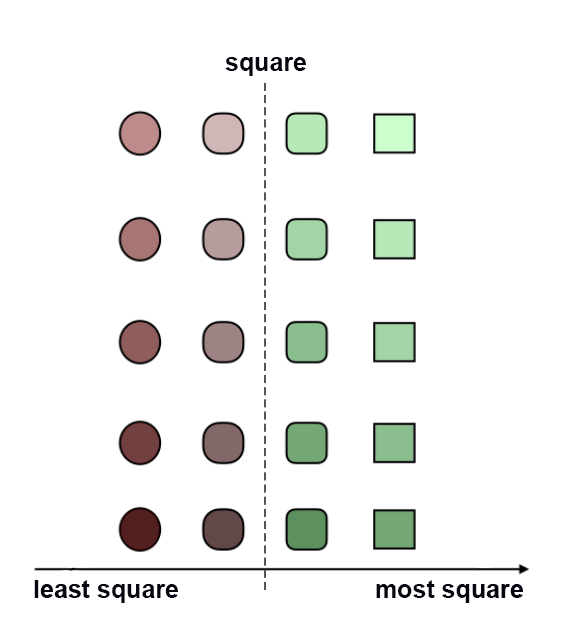
\includegraphics[width=250px]{images/Toyhyperplane1Direction.png}
	\centering
	\caption{An example of a hyper-plane in a toy domain of shapes. The hyper-plane for the word square is the dotted line. Green shapes are positive examples and red shapes are negative examples. \hmark{The arrow along the bottom of the figure indicates the corresponding direction. Those shapes far from  the hyper-plane on the right (positively classified) side of  the direction are more square than those in the opposite direction. }}\label{ch1:introhyp}
\end{figure}

\hmark{These kind of} directions in document embedding models\hmark{, that go from documents that least represent a semantically meaningful word to those that most represent it,} can be useful in a wide variety of applications. \hmark{The most immediate example is being used as features in a simple interpretable classifier, for example in a recommendation system, a movie could be recommended because it is "Scary", "Bloody" and "Funny".} \hmark{Another  example} is  that they allow for a natural way to implement critique-based recommendation systems, where users can specify how their desired result should relate to a given set of suggestions \cite{Viappiani2006}. For instance, Vig et al \cite{Vig2014} propose a movie recommendation system in which the user can specify that they want to see suggestions for movies that are "similar to this one, but scarier". If the direction of being scary \hmark{is captured as a semantic feature}, such critiques can be addressed in a straightforward way. Similarly, in \cite{Kovashka} a system was developed that can find "shoes like these but shinier", based on a document embedding model that was derived from visual features. Semantic search systems can use such directions to interpret queries involving gradual and possibly ill-defined features, such as "\emph{popular} holiday destinations in Europe" \cite{Jameel}. While features such as popularity are typically not encoded in traditional knowledge bases, they can often be represented as document embedding model directions.% Directions can also be used in interpretable classifiers, for example, Derrac and Schockaert \cite{Derrac2015} learned rule based classifiers from ranks induced by the feature directions.

% NEEDS REWRITE
% How a decision tree would work with these semantic features is like this...
% Explanation of the labels and what they mean
% A one-depth decision tree could perform well with a key concept identified for example




% A low-depth decision tree is a prototypical example of a simple interpretable classifier. Performance in a low-depth decision tree relative to the full representation is used for evaluation, as this demonstrates that information in the original vector space has  been retained, and that the features are semantic, as they can sufficiently capture key domain tasks with a small number of features. 
 %good these semantic features are  is evaluated by how well  low-depth Decision Trees perform on key classification tasks in the domain when using these semantic features as input. %As well as demonstrating the use of these features in an interpretable classifier, it can be understood that if, e.g.\ a one-depth decision tree performs well on a key domain task then the representation is capturing a key feature in the domain, as a one-depth decision tree can only use a single semantic feature.  Similarly, in a tree limited to a depth of two, only a few features can be used, so to achieve good classification results, the features must capture particularly important meaning in the domain. An example of a low-depth  Decision Tree, classifying if a movie is a "Sports" movie, is shown below in Figure \ref{ch1:DecisionTree}. To give another example, when classifying if a movie belongs to the Horror genre, strong performance of a depth-2 decision tree suggests that the semantic features are used in the tree that are highly predictive (individually or jointly) of this class, e.g.\ features like "Scary" or "Bloody".



%Decision Trees have nodes that correspond to features, so if these features are simple and easy to understand then the tree is also interpretable \cite{Ustun2014}. 

%\hmark{The intention of this thesis is to post-process existing vector-space representations, disentangling the meaning they represent into semantic features. Relevant semantic features for classification can enable simple interpretable classifiers to perform well, without complexity that may be difficult to navigate without an expert user.  Low-depth decision trees are a prototypical example of such a simple interpretable classifier. 
% This chpater proceeds as follows...
 \hmark{Although the semantic features derived from vector space embeddings do have labels, the intent of this thesis is not to optimize these labels for interpretability. Rather, the intention of this thesis is to develop methods that can transform a given vector space representation, such that components of the resulting vectors  correspond to semantically meaningful (i.e.\ predictive) properties from the considered domain. Such a representation is called "disentangled" - a representation composed of these properties is a disentangled representation.  In Figure \ref{introdectree}, an example of a decision tree that uses the semantic features obtained in this thesis limited to a depth of three is shown. This example is from a domain where text documents are movies, represented by a concatenation of movie reviews. The task is to classify the genre of the movie, and this tree classifies if a movie is a sports movie using semantic features derived from a vector space embedding.}

\begin{figure}[t]
\label{introdectree}
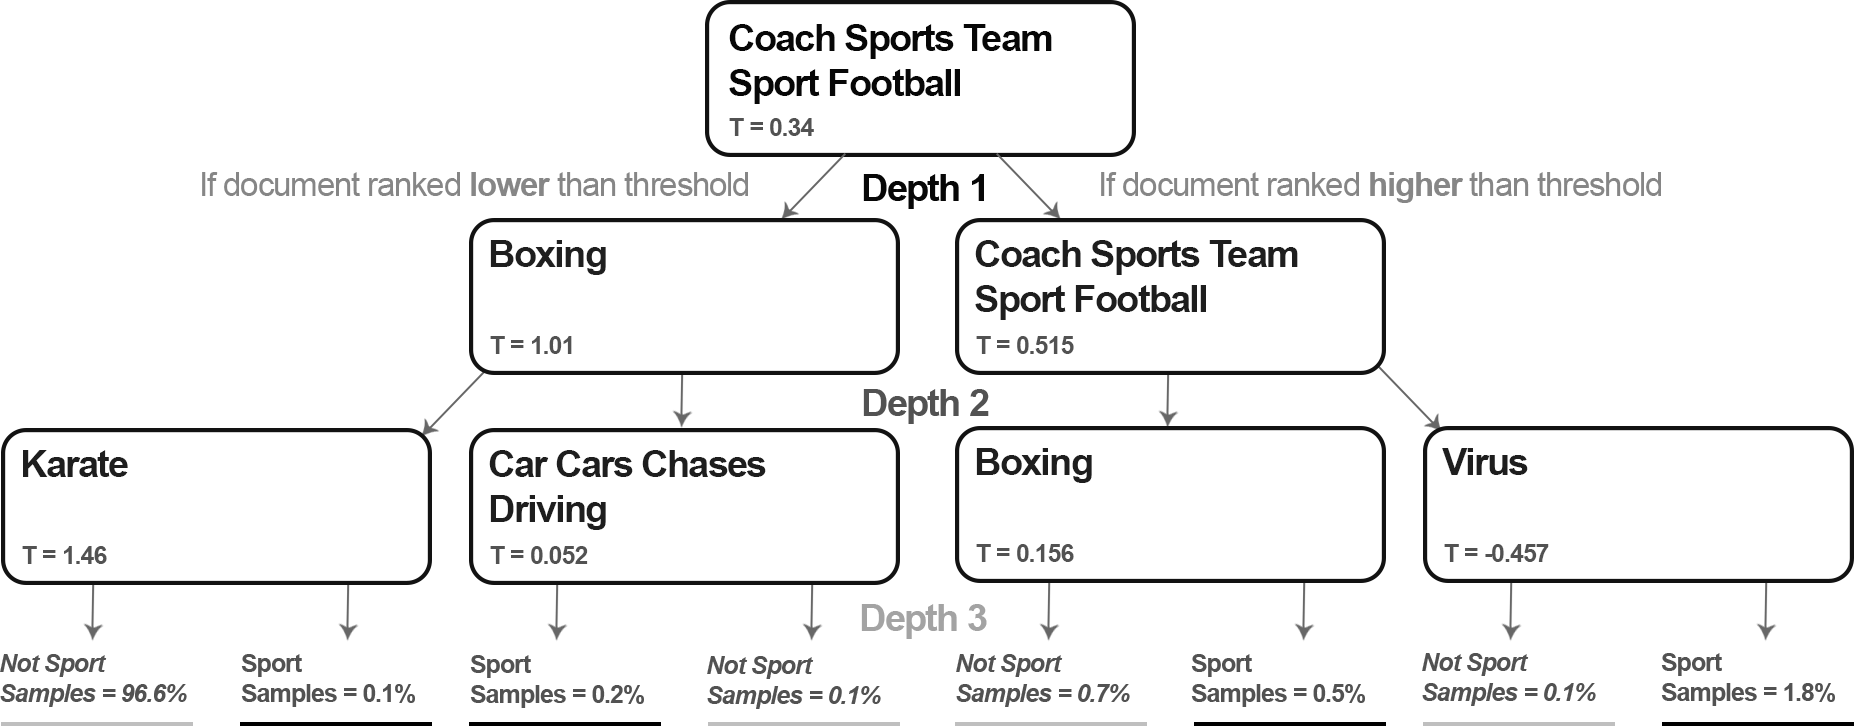
\includegraphics[width=450px]{images/decision_tree_ex.png}
\centering
\caption{An example of a Decision Tree classifying if a movie is in the "Sports" genre. Here,  decision tree nodes use features that capture properties of the domain. These properties are represented by keywords or clusters of keywords.  "Coach Sports Team Sport Football" is a cluster of keywords, that refers to the property in the domain of sports and sport, described using those words and related words like coaches and teams. This  property is extremely useful for classifying if the movie is in the "Sport" genre, and as such is the first node of the tree. Other nodes, like "Virus" apply to only a very small number of samples.}\label{ch1:DecisionTree}
\end{figure}

  This chapter continues as follows: In Section \ref{ch1:hyp} the research hypothesis for the thesis is posed. This is followed by an introduction of three research questions in Section \ref{ch2:rq}, each corresponding to a chapter in the thesis. The contributions of each chapter are  then described in Section \ref{ch2:con}, and the structure of the thesis is laid out in Section \ref{ch1:ths}. 

%%%%%%%%% Disentanglement stuff
%There are a variety of existing approaches to obtain semantic features, historically  Principal Component Analysis has been used to obtain features of facial images \cite{OToole1993}, and more recently Bengio \cite{Bengio2012} identified a desirable property for unsupervised representation learning called "disentanglement". Disentanglement, to "disentangle" factors of the domain that account for variation in the examples, has been used in a variety of domains, in particular in by adjusting the learning methods of particular neural networks e.g.\ in a domain of handwritten digits images,  separate  features are obtained that represent the  "style" of the digit, and the  digit that was written \cite{Chen2016}. In the case of text domains,  a representation was  learned that  has  separate features for the sentiment of the text and the  content  of the text  \cite{John2019}, and in a medical text domain a representation was  learned with features corresponding to key medical aspects\cite{Banner}. } 


%\hmark{Although the intention of disentanglement is similar to that of this thesis, it is typically intrinsically linked to  a neural network structure, like a Generative Adversarial Network, and obtained by adjusting the learning method by e.g.\ requiring features to be independent from each other \cite{Banner}  \cite{Paige2016}. Other approaches to obtain semantic features, for example word vector representations, achieve sparse representations with semantic features by e.g.\ adapting matrix factorization to include sparsity constraints \cite{Murphy}. Our approach has its own focus in two main ways. The first is that this method  obtains semantic features from text documents, and the second is that this thesis focuses on  post-processing existing vector spaces. In particular, this is done by identifying  \textit{semantic relations} in the existing spatial representation and obtaining semantic features from them in an entirely unsupervised way. }





%One way to obtain a representation of the data that results in strong performance is feature engineering [cite], integrating encoded domain knowledge [cite], or using experts to validate the features [cite].  Manually hand-crafting or improving features takes time and knowledge that is not available for many domains, and so methods have been developed to learn features from data without the need of hand-labelling or encoding expert knowledge [cite].

% What are vector spaces? Why are they used? Why are they important and what are they a part of? What are their disadvantages?




%




% What is disentanglement? How does it relate to machine-learning feature Interpretability?  Why is it important?

 % and overlapping regions occur that correspond to properties of the domain (e.g.\ "tasty", "acidic", "bitter", "exotic"). Below, an example is shown of such a vector space.
 
%



%







%\hmark{This use of low-depth decision trees clarifies our aims. One aim is semantic features, which are validated through the classification of key domain tasks using a low-depth decision tree, and the second aim is for these semantic features to be useful for a simple interpretable classifier, which is validated by achieving strong performance without complexity. The idea of a disentangled representation of semantic features  is linked to the objective of interpretability.} 



%Other work which has taken advantage of directions in vector spaces has relied on word embeddings (See Section \ref{bg:WordVectors}). For instance,  \cite{gupta2015distributional} found that features of countries, such as their GDP, fertility rate or even level of CO$_2$ emissions, can be predicted from word embeddings using a linear regression model.   In \cite{kim2013deriving} directional vectors in word embeddings were found that correspond to adjectival scales (e.g.\ bad $<$ okay $<$ good $<$ excellent) while \cite{Rothe2016} found directions indicating lexical features such as the frequency of occurrence and polarity of words.

 %and potentially leading to better generalization, increasing the potential for transfer learning, and resulting in more efficient unsupervised learning  \cite{Banner}  \cite{Paige2016}.   





%Firstly, there are not many approaches that can induce disentangled representations in the domain of text, as 

%"Thus far in NLP, learned distributed represen-
%tations have, with few exceptions (Ruder et al., 2016; He et al., 2017; Zhang et al., 2017), been en- tangled: they indiscriminately encode all aspects of texts. Rather than representing text via a mono- lithic vector, we propose to estimate multiple em- beddings that capture complementary aspects of texts, drawing inspiration from the ML in vision community (Whitney, 2016; Veit et al., 2017a)" \cite{Banner}

%Benefits of disentanglement: Knowing if the model will generalize, transfer learning, more effiicent training when supervised objectivers are not aviavlalb,e  









%Methods that obtain interpretable representations include topic modelling with e.g.\ Latent Dirchlet Allocation (LDA), Negative Matrix Factorization (NMF), among others. 


% What does this thesis do to address that specific case?

% that by separating the key properties of the domain into features,
%The advantage of disentangled representations in this regard is that if the properties of disentangled representations are indeed distinct important concepts in the domain, then that is a first step towards a representation where each feature can be understood by humans. From that representation,  effective machine-learning models can be learned that can explain themselves using these features. However, 

%sHowever, these methods lack the flexibility and broad usage of vector spaces, which are applied in a variety of tasks and are a primary component of neural networks, a method that achieves state-of-the-art in many tasks using text data and in other domains.  

%This thesis offers a new approach for obtaining good disentangled representations, crucially being unsupervised, applied in the text domain, and used as a post-processing step on existing vector space representations. From these features, standard requirements like clustering, classification using simple classifiers, and understanding domains can be achieved, while using the information stored in a representation learned using a large volume of data from e.g.\ a complicated neural network architecture. 

\section{Hypothesis}\label{ch1:hyp} 

%Research hypothesis is the start-  don't give it all away - we dont know what we are doing
%(The previous work no clear rhyme or reason to what works)
%Use "disentangled" not "interpretable" because we are not concerned with labels
%In particular, claiming they are "interpretable" doesn't make sense 
%Provide a useful inductive bias to classifiers, across a range of domains and a range of different vector spaces
%High bias, less noise more robust beause it can only use those features
%Linear classifiers are robust because they can only find things that are linear
% - What is the best way to use linear models to  obtain a disentangled representation semantic features by using words and a linear model
%Question 2: Useful qualitative insights into the characteristics of the layers of neural network models
%Question 3: How can the quality of the features be improved by fine-tuning the vector space

%Vector spaces of text documents encode semantic relationships spatially, e.g.\ in a domain where documents are amazon product reviews, a vector space that is successful at sentiment analysis will be organized such that documents that are negative (i.e. a one-star review) about the product are distant from those that are positive (i.e. a five-star review), and there will be reviews inbetween (two, three or four star reviews). 

\hmark{Semantically meaningful features can be obtained from vector space representations of documents. These features are sufficiently predictive to be useful for simple interpretable classifiers, of which low-depth decision trees are a prototypical example, allowing for a performance that is close to the performance of an unbounded decision tree. Further, when these feature are obtained from neural network hidden layers, they can provide valuable insights into  aspects of the domain that the neural network has learned. }



%Vector space models of text documents can be re-organized into interpretable feature representations. These interpretable feature representations are useful when used in simple interpretable classifiers of key domain tasks, as their features correspond to important properties in the domain. They are effective in multiple domains and can be derived from many types of vector-space. These interpretable feature representations can be made more accurate to domain knowledge and more interpretable with simple unsupervised procedures that ensure they more closely match a bag-of-words.

\section{Research Questions} \label{ch2:rq}

\textbf{Question 1:} \hmark{Can meaningful semantic features be characterised as directions across a wide range of vector space encodings and domains, and do these semantic features allow us to learn effective low-depth decision trees?}





\textbf{Question 2:} \hmark{Can semantic features be obtained to describe the hidden layers of neural networks, and to what extent can these features be used to  investigate  the characteristics of   different neural networks?}

\hmark{These first two questions focus on obtaining semantic features. However, this is not the intention of the final research question. Instead, this question looks at how to improve existing semantic features. In particular, by using a neural network to fine-tune the initial vector space embedding so that the directions contained within it are better suited for use as semantic features.}

\textbf{Question 3:} \hmark{Is it possible to obtain higher-quality semantic features in an unsupervised way by fine-tuning the initial vector space?}

\section{Contributions} \label{ch2:con}  

In the work by Schockaert and Derrac  \cite{Derrac2015}, only three domains were investigated  and all results were based on the same document embedding model. Further, the method was evaluated with fixed hyper-parameters using a rule-based classifier.  \hmark{In Chapter \ref{ch3} we propose a methodology for quantitatively validating variants of the method by Derrac \cite{Derrac2015}, by using low-depth Decision Trees, limited to a depth of one, two or three. Their method is subject to} an extensive quantitative and qualitative evaluation using data from five different domains\hmark{, and vector space embeddings  derived from a variety of document embedding methods. This is important to confirm the generality of the results from \cite{Derrac2015}.}  %\hmark{It is found that low-depth decision trees perform just as well as more complex decision trees in most cases, and indeed outperform complex decision trees in a few select cases.} 


In Chapter \ref{ch4}\hmark{,} the method \hmark{from} Chapter \ref{ch3} \hmark{ is used to obtain semantic representations from  the hidden layers of neural networks}, \hmark{in particular} feed-forward networks and auto-encoders. Specifically, the output of the activation values of the hidden layers  of the trained models are viewed as vector space representations,  and  disentangled feature representations are derived from them. Feed-forward networks are trained on supervised data to classify key domain tasks, and the disentangled feature representations derived from these feed-forward networks are quantitatively tested using depth-3 decision trees. The predictive performance of these decision trees is compared to the neural networks, and it is found that not much predictive performance is lost in most cases, and in one case, the disentangled feature representation obtained from the neural network when used as input to low-depth decision trees  out-performs the neural network it was learned from.  Further, characteristics of feed-forward networks are identified, in particular that they represent new semantic features that are more relevant to the class. \hmark{ However, the same experiment repeated for the stacked, meaning multi-layered, auto-encoder yielded a negative result.} \hmark{Furthermore,} A method is introduced to induce rules that describe relationships between semantic features from each layer, and the application of this method to  better explain how the neural network represents information is explored. This work was published in NeSy 16, the Eleventh International Workshop on Neural-Symbolic Learning and Reasoning.
%  Following this, a qualitative investigation is conducted of  auto-encoder features and it is found that the words used as features become increasingly frequent the deeper the layer of the auto-encoder they were derived from.} 





In Chapter \ref{ch5} we identify an issue with the use of the  centred objective used to build the vector space embedding. Specifically, although the vector spaces can be re-organized into meaningful directions, the similarity objective can sometimes be counterproductive. An example of this in a two-dimensional toy domain is shown in Figure \ref{ch1:toyExample}, where the similarity objective results in an outlier. Following this, a method is introduced to fine-tune the vector space, improving the directions in the vector space embedding at the expense of modelling similarity. First, Positive Pointwise Mutual Information (PPMI) scores for the words that label the interpretable features are obtained. Then, a target ranking for each feature is found by using isotonic regression to obtain values in between the PPMI scores and the rankings of the documents. This target ranking is used to train a single layer neural network with a non-linear activation function that attempts to match the rankings of documents to the target ranking. The intention is not to achieve 100\% accuracy, but instead to rearrange the rankings so that similarity based information is de-prioritized if it allows us to learn more meaningful directions. \hmark{This results in a performance increase in low-depth decision trees for a variety of configurations and tasks, with some exceptions, when these fine-tuned spaces are used as input.} A qualitative investigation shows that the document rankings become more specific and meaningful for the features. This work was published in The SIGNLL Conference on Computational Natural Language Learning (CoNLL) 2018.

\begin{figure}
	\centering
	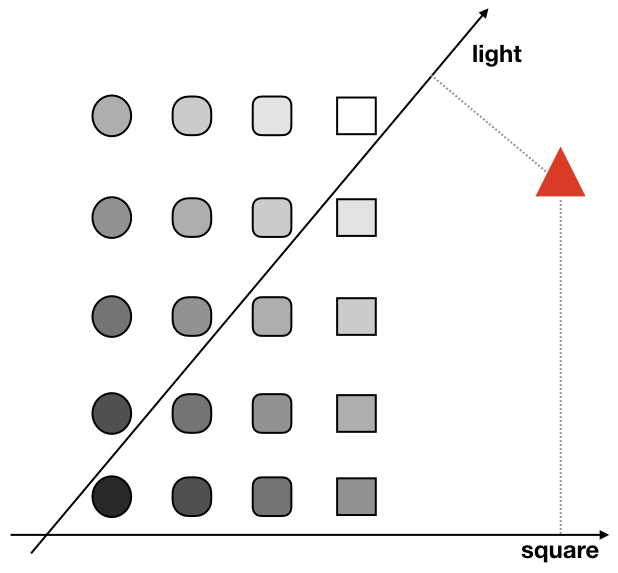
\includegraphics[width=180pt]{images/shapes}
	\caption{Toy example showing the effect of outliers in a two-dimensional embedding of geometric shapes}
	\label{ch1:toyExample}
\end{figure}

%In particular, we use this method of building a representation of entities as a way to convert a vector space into an interpretable representation, for use in an interpretable classifier. The reason that we chose this representation to expand on is because by representing each entity $e$ with a vector $v$ that corresponds to a ranking $r$, the meaning of each dimension is distinct, and we are able to find labels composed of clusters of words for these dimensions. Here, we make the distinction between a property and a word, a property is a natural property of the space that exists in terms of a ranking of entities, and words are the labels we use to describe this property.

%%% HYPOTHESIS


% Introduction to the internet, data, basic text representations
% Introduction to machine learning, benefits of data for machine learning, machine learning representations
% Problems with machine learning, interpretability, lack of interpretability in machine learningg
% We introduce a series of methods for transforming uninterpretable machine learning representations into interpretable ones
% Finding directions in vector spaces and using those to produce interpretable representations
% Fine-tuning these directions to get a better result
% Interpreting and investigating neural networks with these directions


%This brings up an essential point: When using a semantic space, are we taking advantage of relationships that are discriminative or incorrect? The danger of relying on these spaces and the models that use them has greatly affected their adoption in critical application areas like medicine, %Citation needed
%and has raised legal concerns about their application in e.g.\ determining if someone is suitable for a loan. 


\section{Thesis Structure} \label{ch1:ths}

\begin{itemize}
	\item \textbf{Chapter \ref{ch2}} gives an overview of methods for processing unstructured text data, standard machine-learning classifiers, and it provides a background \hmark{on other methods to discover semantic features and on related work in interpretability}.
	\item \textbf{Chapter \ref{ch2.5}} introduces and explains the datasets used in this thesis, as well as \hmark{explaining} the hyper-parameters  used for the machine-learning models in this thesis.
	\item \textbf{Chapter \ref{ch3}} provides a comprehensive quantitative and qualitative analysis of the method introduced by Derrac \cite{Derrac2015}, across a much broader group of domains, tasks, and vector space embedding methods. This section introduces the use of low-depth decision trees as a mechanism for evaluating the quality of the learned semantic features.  \hmark{Additionally, for the sake of completeness, variations of the method are introduced, with scoring functions that were previously not used, such as  NDCG, F1-score and accuracy. Standard k-means is used as an additional clustering algorithm that provides a reference point to the variation of k-means used in the original work. All variations, parameters, entity embedding methods and domains are comprehensively analysed and compared. }
	\item \textbf{Chapter \ref{ch4}} qualitatively investigates the use and application of the method in Chapter \ref{ch3} to neural networks, in particular feed-forward networks and auto-encoders. A rule-based classifier is used to connect properties between layers of an auto-encoder.
	\item \textbf{Chapter \ref{ch5}} introduces a  method to improve the interpretable feature representation by prioritizing these features over the similarity information that is captured in the vector space.
	\item \textbf{Chapter \ref{ch6}} provides conclusions on the contributions of this thesis and outlines a number of possible avenues for future work.
\end{itemize}


\section{Summary}

Vector space representations of text documents are common in Natural Language Processing (NLP). However, their features are typically not interpretable.  There is an increasing need for suitable solutions to interpretability in NLP and machine-learning. A prototypical example of a simple interpretable classifier is a low-depth decision tree. A low-depth decision tree is effective when it  semantic features are used as input. These features  correspond to properties of the domain that are suitable for the class, e.g.\ A property that represents the property of a movie being "Bloody" when classifying if a movie is a "Horror". This thesis studies methods for inducing such semantic features from a variety of vector space encodings of documents, including neural networks.





%Shouldn't this be a summary of the chapter, rather than a summary of the thesis? If so, the story should rather be:

%* Vector space representations of documents are common in NLP. While they perform well, they are also difficult to interpret
%* Interpretability is an increasingly important challenge for NLP and ML, with small decision trees a prototypical example of an %interpretable classifier.
%* But such classifiers can only be effective if they have access to the right semantic features.
%* The aim of your thesis is to study methods for inducing such features from a variety of vector space encodings of documents.



% Our work is...

%\section{Relationships}

%Vector spaces are representations that reduce the dimensionality of sparse representations like bag-of-words into dense spaces where semantic relationships e.g.\ two movies being similar to one another, are represented spatially. However, upon reducing this dimensionality the features are no longer interpretable.  One way to interpret what these vector spaces mean follows Conceptual Spaces \ref{????}, where entities in the domain e.g.\ movies in a domain of movie reviews are represented as points, and properties in the domain are represented as convex regions. The work in Chapter \ref{ch3} details a process where the vector space is transformed so that these properties are used as features, creating an interpretable but dense representation. The introduction goes into further detail about these properties.
% Conceptual spaces

% properties

% using properties as features

%\section{Contributions}\label{ch1:contributions}

% chapter 3 does this
%etc

%\section{Representations}




%\section{Motivation}
%What is text? How is it motivating?

%What are the desiradata of a good representation?
% Unsupervised


%One task of Natural Language Processing is to obtain this semantic understanding from text by obtaining a machine-readable representation that contains domain knowledge. A basic approach to obtain a representation of this text is to represent entities (e.g.\ reviews, text-posts) by the frequency of their words, see \ref{Bag-of-words-example}.

%\begin{figure}[t]
%	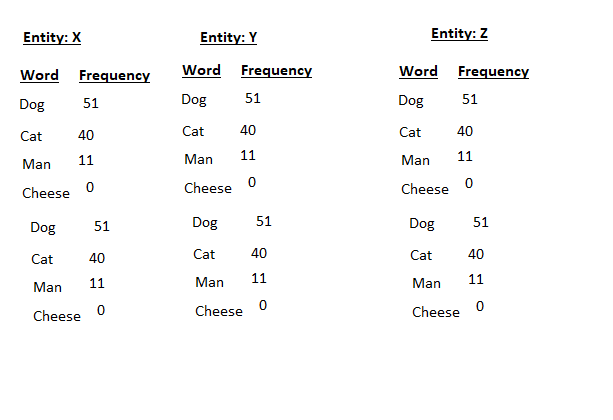
\includegraphics[width=\textwidth]{images/bowbowbow.png}
%	\centering
%	\caption{Bag-of-words  }\label{Bag-of-words-example}
%\end{figure}


 %Below, we show a review with its associated properties labelled.

%\begin{figure}[t]
%	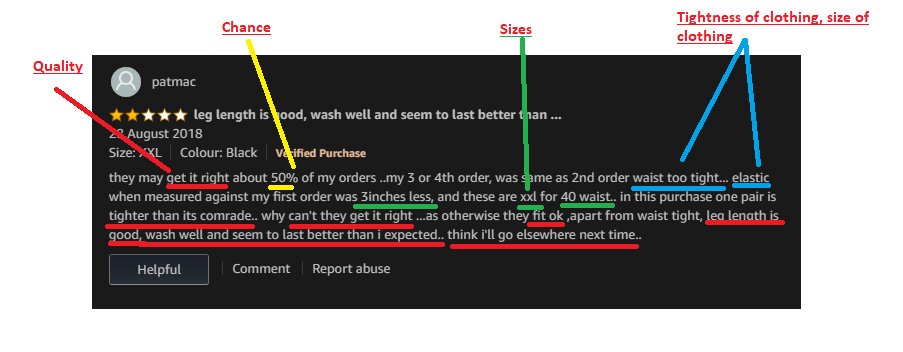
\includegraphics[width=\textwidth]{images/leg_length.png}
%	\centering
%	\caption{Example properties  }\label{IntroDecisionTree}
%\end{figure}

%\subsection{Machine Learning}
% what is machine learning? why do i care?


% Granular
%We can understand these properties to have a degree to which they apply, for example the size of the clothing might be "XXL", "XL", "L", "M" or "S", or the quality may be "Very good", "Good", "Ok", "Bad" or "Very bad". For the former, we may rely on the metadata available from the site itself, but for the latter the way to obtain this information is less clear. Although we may infer that the rating has some indication of these properties, it does not describe the properties or the degree to which the review refers to them. %This kind of information is valuable for making sense of the world of unstructured text, and has broad applications, e.g.\ The most immediate example is perhaps that they allow for a natural way to implement critique-based recommendation systems, where users can specify how their desired result should relate to a given set of suggestions \cite{viappiani2006preference}. For instance, \cite{Vig:2012:TGE:2362394.2362395} propose a movie recommendation system in which the user can specify that they want to see suggestions for movies that are "similar to this one, but scarier". If the property of being scary is adequately modelled as a direction in a semantic space of movies, such critiques can be addressed in a straightforward way. Similarly, in \cite{kovashka2012whittlesearch} a system was developed that can find "shoes like these but shinier", based on a semantic space representation that was derived from visual features. Semantic search systems can use such directions to interpret queries involving gradual and possibly ill-defined features, such as "\emph{popular} holiday destinations in Europe" \cite{DBLP:conf/sigir/JameelBS17}. While features such as popularity are typically not encoded in traditional knowledge bases, they can often be represented as semantic space directions.  %Copied from CONLL

%\subsection{Directions}\label{intro:directions}


%However, manually labelling these properties and the degrees to which entities (e.g.\ reviews, text-posts) have them is extremely time-consuming. 

%A potentially ideal system would be as follows: We collect large amounts of unstructured text data, separated into domains, and obtain the properties of each domain from this data, and rank entities on the degree to which they have these properties. In this way, properties would be understood on a scale built from the domain directly, so that each domain has its own meanings for words according to their own idiosyncrasies. As the process does not require any manual labelling the quality of these properties could be improved simply by obtaining more data. Further, as we are learning from unstructured data, not only would this allow us to understand the data in terms of what we know, but it would also introduce us to new ideas that we may not have previously understood. This kind of representation also has value in application to Machine Learning tasks. If we can separate the semantics of the space linearly into properties, we are able to learn simple linear classifiers that perform well. 

%Simple linear classifiers built from a representation composed of rankings on properties have an additional benefit of being more understandable.


% Natural clustering
% Semantically distinct
% Interpretable
% Curse of dimensionality
% Generalizability ("shared factors across many tasks" \cite{Bengio2012})

%What is machine learning? What are its advantages? How is it motivating?

%What are the problems with machine learning? How is it motivating?


%What is domain-specific? What is domain knowledge? %On the web there is a large volume of raw text data, e.g.\ Reviews of products, movies, anime, books, music, social posts by individuals, self-descriptive text about a website or product, and so on. These can be categorized into domains; each domain has its own quirks, knowledge, and method of being brought about. Although a movie review may sound similar to a book review, they typically differ hugely in the distribution of words used.

%

%\section{Interpretability}\label{ch1:interpret}

%What is interpretability? How is the value of interpretability measured in the real world?

%How can we meet the needs of the real world?  Is it transparancy, the system having easy to understnad components, etc... what  are the different views on what an interpretabile system is?

%What specific interpretability task are we trying to solve? How do we define interpretability? Why is it valuable, where is it used? What was the hypothesis/research question?
%%What are distributional models?
%Most successful approaches in recent times, like vector-spaces, word-vectors, and others, rely on the distributional model of semantics. This model relies on encoding unstructured text e.g.\ of a movie review, as a vector, where each dimension corresponds to how frequent each word is, we are able to calculate how similar the entities are, e.g.\ we know that if two movies have a similar distribution of words in their reviews, like frequent use of the word 'scary', or 'horror', then they would have a higher similarity value. These models, also known as 'semantic spaces' encode this similarity information spatially.

%Semantic relationships can be obtained from semantic spaces. 

%applications/need for good interpretability:

%What is a conceptual space? What are entities?  What are properties? What is commonsense reasoning?
%properties of an interpretable classifier:
%\begin{itemize}
%	\item Complexity: 'the magic number is seven plus or minus two' \cite{Saaty2003} also has many positive effects for its users, like lower response times \cite{Narayanan2018, Huysmans2011}, better question answering and confidence for logical problem questions \cite{Huysmans2011} and higher satisfaction \cite{Narayanan2018}.
%	\item Transparancy: 
%	\item Explainability: 
%	\item Generalizability:
%\end{itemize}


%X%X%What is a symbolic approach?  %One approach to making sense of these domains is to produce rules from expert knowledge. An expert in movies would tell you that if the review talks about it being a "cannibal horror film", we can understand that it is likely a scary movie and is related to the original 'Cannibal Holocaust' movie. Encoding this kind of knowledge is difficult, time-consuming, and hard to automate reliably.

%Properties, entities, the benefits and application of a representation formed of these

%Basic introduction to directions, explanation of the utility and application of our approach
%\section{Thesis Overview / Contributions}

%What were our objectives starting out? 
%What are our intentions with how the work in the thesis will be used?
%What are our contributions?
%%What are our aims for this chapter? What do we overall want to do? (Already kind-of said in Chapter 1, but worth repeating I guess in some form)
%In \ref{Chapter3}, we introduce a pipeline that starts with unstructured text, and ends with an interpretable representation of entities represented by properties labelled by clusters of words. Further, we demonstrate the applicability of these representations in a simple Decision Tree that uses just a few of these properties to classify entities. In Figure \ref{ExamplesWithTree}, we show some example movie entities, their associated properties, and a Decision Tree classifying whether or not they are a Horror movie. 

